\documentclass[12pt]{exam}
\usepackage[phy]{template-for-exam}
\usepackage{tikz,ifthen,multicol,graphicx}
\footer{}{}{}
\header{}{}{}
\shadedsolutions
%\printanswers



\begin{document}

\Large

\def\mystrut{\protect\rule[-2.2ex]{0ex}{2.2ex}} 
\qformat{ \textbf{Task \#\thequestion}
  \ifthenelse{\equal{\thequestion}{\thequestiontitle}}
    {}
    {: \emph{\thequestiontitle}}
  \mystrut  \hfill}


\begin{questions}

\vspace*{\stretch{1}}

\question
  You pedal your 75-kg bike with a force of 423 Newtons.  You accelerate at a rate of 1.8 m/s$^2$.  What is the force of friction?  Ignore Air Resistance

  \begin{solution}
    288 N
  \end{solution}


\vs \hrule \vs

\question
  Before opening her parachute, a 57-kg skydiver experiences 457 N of air drag.  What is the magnitude of her downward acceleration?
  
  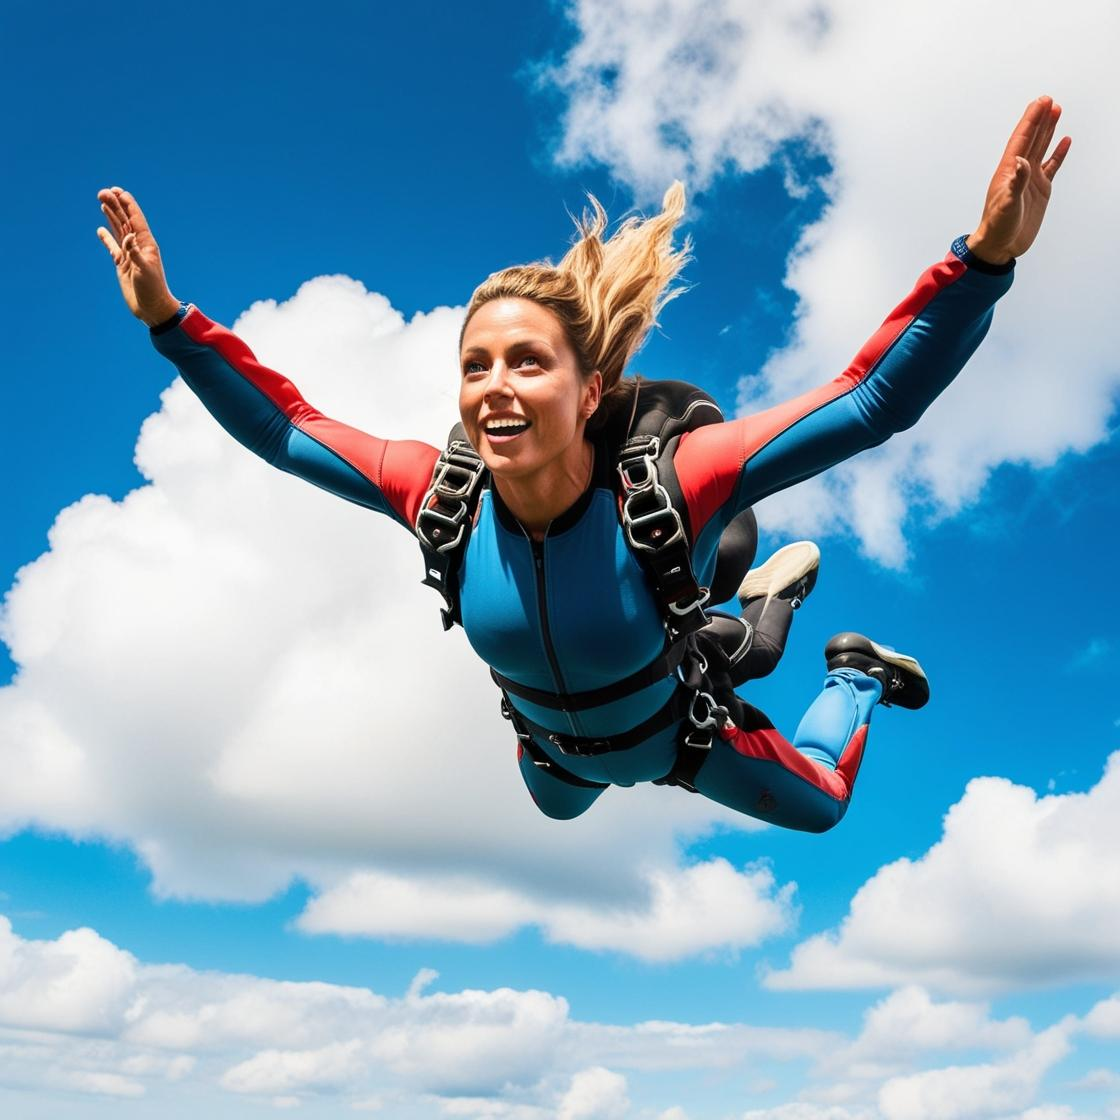
\includegraphics[height=4cm]{skydiver.jpg}
  \begin{solution}
      $F_{NET}=101.6$ N; $a=1.78$ m/s$^2$;

      Extension: A few moments later, she reaches terminal velocity, which means she is no longer accelerating.  What is the air drag force at terminal velocity?
  \end{solution}

\vs \hrule \vs



\question
  A piano is lifted by a crane with a force of 12,500 N.  It accelerates at a rate of 1.3 m/s$^2$.  What is the mass of the piano?

  \begin{solution}
    1126.1 kg
  \end{solution}

\vs 

\end{questions}




\end{document}